% ======================================================================
%  Fusklapp 732G53 – Linjär regression (tentamen)
%  Tillåtet: två A4-blad dubbelsidigt => exakt 4 sidor (A4 liggande).
%  Bygger på kurssidan https://hietalai.github.io/statistics-in-r/
%  (Del II Regressionsanalys, kap. 1-11) samt tentor 2024-10-25,
%  2025-01-20, 2025-02-28 och 2025-10-23.
%  Kompilera: pdflatex fusklapp_732G53.tex  (kör två gånger för korsreferenser)
% ======================================================================
\documentclass[8pt]{extarticle}
\usepackage[a4paper,landscape,margin=6mm,includehead,headheight=9pt,headsep=2pt]{geometry}
\usepackage[T1]{fontenc}
\usepackage[utf8]{inputenc}
\usepackage[swedish,shorthands=off]{babel}
\usepackage{mathptmx}
\usepackage[scaled=0.92]{helvet}
\usepackage{amsmath,amssymb}
\usepackage{multicol}
\usepackage[dvipsnames]{xcolor}
\usepackage{enumitem}
\usepackage{booktabs}
\usepackage{array,tabularx}
\usepackage{tikz}
\usepackage{newunicodechar}
\usepackage{pifont}
\usepackage{microtype}
\usepackage{fancyhdr}

\newunicodechar{⇒}{\ensuremath{\Rightarrow}}
\newunicodechar{⇔}{\ensuremath{\Leftrightarrow}}
\newunicodechar{→}{\ensuremath{\rightarrow}}
\newunicodechar{≡}{\ensuremath{\equiv}}
\newunicodechar{✓}{\textcolor{OliveGreen}{\ding{51}}}
\newunicodechar{✗}{\textcolor{BrickRed}{\ding{55}}}
\newunicodechar{≈}{\ensuremath{\approx}}
\newunicodechar{≠}{\ensuremath{\neq}}
\newunicodechar{≤}{\ensuremath{\le}}
\newunicodechar{≥}{\ensuremath{\ge}}
\newunicodechar{×}{\ensuremath{\times}}
\newunicodechar{−}{\ensuremath{-}}

% ---------- utseende ----------
\pagestyle{fancy}\fancyhf{}\renewcommand{\headrulewidth}{0pt}
\newcommand{\pagelabel}{\ifcase\value{page}\or GRUNDER \& RÄKNA FÖR HAND\or INFERENS \& TOLKNING\or DIAGNOSTIK \& MODELLVAL\or TENTASTRATEGI, SANT/FALSKT \& TEORISVAR\fi}
\newcommand{\tsq}[1]{\textcolor{#1}{\rule{5pt}{5pt}}}% temafärgad ruta (sidhuvud, register)
\fancyhead[L]{\fontsize{6.5}{7}\selectfont\sffamily\textcolor{hd}{\textbf{732G53 fusklapp}}\quad\textbf{Sida \thepage/4:} \pagelabel}
\fancyhead[R]{\fontsize{6}{7}\selectfont\sffamily
  \tsq{cGrund}\,Grund\quad\tsq{cRakna}\,Räkna\quad\tsq{cInfer}\,Inferens\quad
  \tsq{cBygg}\,Modellbygge\quad\tsq{cDiag}\,Diagnostik\quad\tsq{cTenta}\,Tenta}
\setlength{\parindent}{0pt}
\setlength{\parskip}{0.6pt}
\setlength{\columnsep}{3.5mm}
\setlength{\columnseprule}{0.2pt}
\setlength{\tabcolsep}{2.5pt}
\setlist{nosep,leftmargin=8pt,labelsep=2pt}
\setlist[itemize]{label=\textcolor{hd}{\textbullet}}
\makeatletter
\g@addto@macro\normalsize{%
  \setlength\abovedisplayskip{1.5pt}\setlength\belowdisplayskip{1.5pt}%
  \setlength\abovedisplayshortskip{0pt}\setlength\belowdisplayshortskip{1pt}}
\makeatother

\definecolor{hd}{HTML}{1F4E79}  % rubriker
\definecolor{ex}{HTML}{9C3D00}  % exempel från tentor
% temafärger (avsnittsrutor, register, sidhuvud)
\definecolor{cGrund}{HTML}{1F4E79} % = hd
\definecolor{cRakna}{HTML}{2E7D32}
\definecolor{cInfer}{HTML}{C2410C}
\definecolor{cBygg}{HTML}{6A1B9A}
\definecolor{cDiag}{HTML}{B71C1C}
\definecolor{cTenta}{HTML}{455A64}
\definecolor{cEnk}{HTML}{00695C}
\newcounter{sect}
% \sect[temafärg]{rubrik}{etikett}: rubriken kan inte hamna ensam sist i en kolumn
\makeatletter
\newcommand{\sect}[3][hd]{\par\vspace{1.5pt}\refstepcounter{sect}\noindent
  \colorbox{#1}{\parbox{\dimexpr\linewidth-2\fboxsep}{\color{white}\sffamily\bfseries
  \thesect\enspace #2}}\label{#3}\par\nobreak\vspace{0.8pt}\@afterheading}
% inga negativa straff vid listor/miljöer => kolumnerna fylls jämnt med \raggedcolumns
\@beginparpenalty=0 \@endparpenalty=0 \@itempenalty=0
\makeatother
\newcommand{\sub}[1]{{\color{hd}\sffamily\bfseries #1}\enspace}
\newcommand{\ex}{{\color{ex}\sffamily\bfseries Ex.}\ }
\newcommand{\obs}{{\color{BrickRed}\sffamily\bfseries OBS!}\ }
\newcommand{\sant}{\textcolor{OliveGreen}{\sffamily\bfseries S}}
\newcommand{\falskt}{\textcolor{BrickRed}{\sffamily\bfseries F}}
\newcommand{\enk}[1]{{\color{cEnk}\sffamily\bfseries Enkelt:} {\itshape #1}}

% ---------- matematik ----------
\newcommand{\SSE}{\mathrm{SSE}}
\newcommand{\SSR}{\mathrm{SSR}}
\newcommand{\SSY}{\mathrm{SSY}}
\newcommand{\MSE}{\mathrm{MSE}}
\newcommand{\MSR}{\mathrm{MSR}}
\newcommand{\SSq}{\mathrm{SS}}
\newcommand{\X}{\mathbf{X}}
\newcommand{\Y}{\mathbf{Y}}
\newcommand{\bb}{\boldsymbol{\beta}}
\newcommand{\bbh}{\hat{\boldsymbol{\beta}}}
\newcommand{\iid}{\overset{\text{iid}}{\sim}}

% ---------- små schematiska residualdiagram ----------
\newlength{\figunit}\setlength{\figunit}{1.07cm}% figurskala (+7 %); nodtextens storlek oförändrad
\newcommand{\miniram}[1]{%
  \draw[gray!60] (0,-0.5) rectangle (1.6,0.5);
  \node[font=\fontsize{5}{5}\selectfont\sffamily,anchor=north] at (0.8,-0.5) {#1};}

\begin{document}

\noindent{\color{hd}\sffamily\bfseries\large 732G53 Linjär regression – fusklapp}\hfill
{\footnotesize \textbf{Notation:} $n$ = antal obs., $k$ = antal förklarande variabler (lutningsparametrar), $p=k+1$ = antal parametrar, $df_E=n-(k+1)$.\quad
Källor: hietalai.github.io/statistics-in-r (Del II) och tentor 2024-10-25 – 2025-10-23.}

\begin{multicols*}{3}
\raggedcolumns

% ======================================================================
\sect[cGrund]{Hitta rätt avsnitt – vanliga tentafrågor}{sec:index}
{\small
\begin{tabular*}{\linewidth}{@{}l@{\hspace{2.5pt}}l@{\extracolsep{\fill}}r@{}}
\tsq{cRakna} & $b_0$, $b_1$, ANOVA, test, KI/PI för hand (enkel regression) & §\ref{sec:slr} (s.\pageref{sec:slr}), §\ref{sec:ex} (s.\pageref{sec:ex})\\
\tsq{cGrund} & Ange/kontrollera antagandena, tolka residualdiagram/QQ-plot & §\ref{sec:modell} (s.\pageref{sec:modell}), §\ref{sec:monster} (s.\pageref{sec:monster})\\
\tsq{cGrund} & OLS-egenskaper, normalekvationer & §\ref{sec:teori} (s.\pageref{sec:teori})\\
\tsq{cInfer} & Hypotesprövningens steg, $p$-värde & §\ref{sec:test} (s.\pageref{sec:test})\\
\tsq{cGrund} & Tolka koefficient, $R^2$, intervall & §\ref{sec:tolk} (s.\pageref{sec:tolk})\\
\tsq{cBygg} & Tolka och testa indikator, interaktion & §\ref{sec:dummy} (s.\pageref{sec:dummy}), §\ref{sec:inter} (s.\pageref{sec:inter})\\
\tsq{cInfer} & Läs R-utskrift, $R^2$ ur ANOVA-tabell, sekventiella SS & §\ref{sec:anova} (s.\pageref{sec:anova}), §\ref{sec:R2} (s.\pageref{sec:R2})\\
\tsq{cInfer} & $F$-test för modellen / $t$-test för en parameter & §\ref{sec:F} (s.\pageref{sec:F}), §\ref{sec:t} (s.\pageref{sec:t})\\
\tsq{cInfer} & Partiellt $F$: kvalitativ variabel, ”kan modellen reduceras?” & §\ref{sec:partF} (s.\pageref{sec:partF})\\
\tsq{cInfer} & Prediktion; flera intervall samtidigt (Bonferroni m.fl.) & §\ref{sec:pred} (s.\pageref{sec:pred}), §\ref{sec:simultan} (s.\pageref{sec:simultan})\\
\tsq{cBygg} & Polynom, transformation, centrering & §\ref{sec:poly} (s.\pageref{sec:poly})\\
\tsq{cDiag} & Leverage, jackknife, DFFITS, Cook's distance & §\ref{sec:infl} (s.\pageref{sec:infl})\\
\tsq{cDiag} & Korrelationsmatris, VIF, multikollinearitet & §\ref{sec:vif} (s.\pageref{sec:vif})\\
\tsq{cGrund} & Confounding, kontrollvariabel, Simpsons paradox & §\ref{sec:design} (s.\pageref{sec:design})\\
\tsq{cBygg} & Välj bästa modell, $C_p$, AIC, validering & §\ref{sec:val} (s.\pageref{sec:val}), §\ref{sec:valj} (s.\pageref{sec:valj})\\
\tsq{cTenta} & Sant/falskt-påståenden; korta svar på teorifrågor & §\ref{sec:sf} (s.\pageref{sec:sf}), §\ref{sec:teorisvar} (s.\pageref{sec:teorisvar})\\
\tsq{cTenta} & Läsa tabellsamlingen ($t$, $F$, $z$); QQ-kvantiler för hand & §\ref{sec:tab} (s.\pageref{sec:tab})
\end{tabular*}}

% ======================================================================
\sect[cGrund]{Modell och antaganden}{sec:modell}
$Y_i=\beta_0+\beta_1X_{i1}+\dots+\beta_kX_{ik}+E_i$,\quad $E_i\iid N(0,\sigma^2)$
\;⇔\; $Y|X\iid N(\mu_{Y|X},\sigma^2)$ med $\mu_{Y|X}=E[Y|X]=\beta_0+\beta_1X_1+\dots$ (väntevärdet saknar felterm).
Skattad modell: $\hat y_i=b_0+b_1x_{i1}+\dots+b_kx_{ik}$ ($b_j=\hat\beta_j$); residual $e_i=y_i-\hat y_i$ skattar $E_i$.
Minsta kvadratmetoden (OLS) väljer $b_j$ som minimerar $\SSE=\sum e_i^2$.

\sub{Antaganden}(1) för varje $X$ finns en slumpvariabel $Y$ med ändligt medelvärde och varians; (2) oberoende observationer; (3) linjäritet: $\mu_{Y|X}$ linjär i parametrarna; (4) lika varians $\sigma^2_{Y|X}\equiv\sigma^2$ (homoskedasticitet); (5) $Y|X$ normalfördelad.
\obs Inget antagande om att $Y$ självt är normalfördelat – kontrollera \emph{residualerna}. Kontrollera antagandena \emph{innan} test/intervall tolkas.

\sub{Kontroll}(✓ = uppfyllt, ✗ = ej uppfyllt)
\begin{itemize}
\item \textbf{Linjäritet} – $e$ mot $\hat y$ (och mot varje $X_j$). ✓ slumpmässig svärm kring 0 utan mönster. ✗ krökt/U-format mönster (även krökt QQ) ⇒ lägg till $X^2$, interaktion, saknad variabel eller transformera.
\item \textbf{Lika varians} – $e$ mot $\hat y$. ✓ jämnbrett band: två parallella linjer längs min/max ramar in punkterna. ✗ tratt/kon (spridningen ökar/minskar med $\hat y$) ⇒ transformera $Y$ ($\ln Y$, $\sqrt Y$).
\item \textbf{Normalfördelning} – histogram och QQ-plot av residualerna. ✓ symmetrisk klockform kring 0; punkterna följer linjen. ✗ skev, flera toppar (saknad grupperingsvariabel), S-form/tunga svansar, extremvärden.
\item \textbf{Oberoende} – $e$ mot observationsordning (linjediagram) + hur data samlats in. ✓ inget mönster (”slump”). ✗ trender/vågor: tidsserier, upprepade mätningar på samma enhet, familjer, närliggande platser.
\end{itemize}
Litet $n$ (t.ex.\ 6): svårt att bedöma – skriv det. \emph{Formulering:} ”Residualerna ser approximativt normalfördelade ut: histogrammet är symmetriskt och klockformat kring 0 och punkterna i QQ-diagrammet följer linjen. Residualerna mot anpassade värden bildar ett jämnbrett band utan mönster ⇒ linjäritet och lika varians verkar uppfyllda.”

\begin{center}
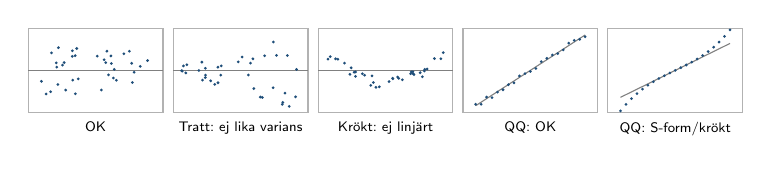
\begin{tikzpicture}[x=\figunit,y=\figunit]
\pgfmathsetseed{11}
\begin{scope}
  \miniram{OK}\draw[gray] (0,0)--(1.6,0);
  \foreach \i in {1,...,36}{\pgfmathsetmacro\xx{0.1+1.4*rnd}\pgfmathsetmacro\yy{0.33*rand}\fill[hd] (\xx,\yy) circle (0.55pt);}
\end{scope}
\begin{scope}[xshift=1.72\figunit]
  \miniram{Tratt: ej lika varians}\draw[gray] (0,0)--(1.6,0);
  \foreach \i in {1,...,36}{\pgfmathsetmacro\xx{0.1+1.4*rnd}\pgfmathsetmacro\yy{(0.03+0.3*\xx)*rand}\fill[hd] (\xx,\yy) circle (0.55pt);}
\end{scope}
\begin{scope}[xshift=3.44\figunit]
  \miniram{Krökt: ej linjärt}\draw[gray] (0,0)--(1.6,0);
  \foreach \i in {1,...,36}{\pgfmathsetmacro\xx{0.1+1.4*rnd}\pgfmathsetmacro\yy{0.75*((\xx-0.8)*(\xx-0.8)-0.2)+0.07*rand}\fill[hd] (\xx,\yy) circle (0.55pt);}
\end{scope}
\begin{scope}[xshift=5.16\figunit]
  \miniram{QQ: OK}\draw[gray] (0.15,-0.42)--(1.45,0.42);
  \foreach \u in {-1,-0.9,...,1.01}{\pgfmathsetmacro\v{\u+0.07*rand}\fill[hd] (0.8+0.65*\u,0.42*\v) circle (0.55pt);}
\end{scope}
\begin{scope}[xshift=6.88\figunit]
  \miniram{QQ: S-form/krökt}\draw[gray] (0.15,-0.32)--(1.45,0.32);
  \foreach \u in {-1,-0.9,...,1.01}{\pgfmathsetmacro\v{\u+0.55*\u*\u*\u}\fill[hd] (0.8+0.65*\u,0.31*\v) circle (0.55pt);}
\end{scope}
\end{tikzpicture}
\end{center}

% ======================================================================
\sect[cGrund]{Läsa QQ-plot och residualmönster}{sec:monster}
\begin{itemize}
\item \textbf{QQ-plot} (observerade mot teoretiska kvantiler): längs linjen ⇒ normalfördelat. Båda ändarna \emph{över} linjen (konvex) ⇒ högerskev; båda \emph{under} (konkav) ⇒ vänsterskev; vänster ände under och höger över (S-form) ⇒ tunga svansar/extremvärden; tvärtom ⇒ lätta svansar; hopp/trappsteg ⇒ grupper. Krökt mönster kan också spegla icke-linjäritet (kurssidan).
\item \textbf{$e$ mot $\hat y$:} två eller flera band ⇒ saknad kategorisk variabel (mod\_2 i tenta 2025-10-23); kors-/solfjädersmönster ⇒ saknad interaktion; enstaka punkt långt från 0 ⇒ möjligt extremvärde (kontrollera standardiserad/jackknife-residual, §\ref{sec:infl}).
\item \textbf{Histogram:} två toppar ⇒ grupper; skevt ⇒ transformera $Y$. \textbf{$e$ mot ordning:} trender/vågor ⇒ beroende.
\end{itemize}

% ======================================================================
\sect[cGrund]{Utforskande analys och spridningsdiagram}{sec:utforska}
\textbf{Rita:} förklarande $X$ på $x$-axeln, respons $Y$ på $y$-axeln, axeltitlar med enhet, rubrik. \textbf{Beskriv fyra saker:} (1) linjärt? (2) positivt/negativt? (3) starkt/svagt? (4) extremvärden? Kvalitativ $X$: fiol-/lådagram per kategori. Responsens histogram behöver \emph{inte} vara normalfördelat.
\textbf{Pearsons $r$} ($-1\le r\le1$) mäter bara \emph{linjära} samband – missvisande vid krökta/icke-monotona samband och vid grupper (Simpsons paradox, §\ref{sec:design}); visualisera alltid. Korrelationsmatris: högt $|r(X_j,Y)|$ ⇒ relevant variabel; högt $|r(X_i,X_j)|$ ⇒ risk för multikollinearitet. Variabeltyper: kvalitativ (nominal-, ordinalskala) → indikatorer; kvantitativ (intervall-, kvotskala).

% ======================================================================
\sect[cRakna]{Enkel linjär regression – räkna för hand}{sec:slr}
\vspace{-3pt}
\begin{align*}
S_{xx}&=\textstyle\sum(x_i-\bar x)^2=\sum x_i^2-(\sum x_i)^2/n\\
S_{yy}&=\SSY=\textstyle\sum(y_i-\bar y)^2=\sum y_i^2-(\sum y_i)^2/n\\
S_{xy}&=\textstyle\sum(x_i-\bar x)(y_i-\bar y)=\sum x_iy_i-\sum x_i\sum y_i/n
\end{align*}
$b_1=\dfrac{S_{xy}}{S_{xx}}$,\quad $b_0=\bar y-b_1\bar x$ \quad (linjen går genom $(\bar x,\bar y)$; $\sum e_i=0$, $\sum x_ie_i=0$)\\[1pt]
$\SSR=b_1S_{xy}=S_{xy}^2/S_{xx}$,\quad $\SSE=S_{yy}-b_1S_{xy}=\sum(y_i-\hat y_i)^2$\\
$s^2=\MSE=\SSE/(n-2)$,\quad $s=\sqrt{\MSE}$ (residualspridning)\\
$r=\dfrac{S_{xy}}{\sqrt{S_{xx}S_{yy}}}$,\quad $R^2=r^2=\dfrac{\SSR}{\SSY}$,\quad $b_1=r\,\dfrac{s_y}{s_x}$\\[1pt]
$s_{b_1}=\dfrac{s}{\sqrt{S_{xx}}}$,\quad $s_{b_0}=s\sqrt{\dfrac1n+\dfrac{\bar x^2}{S_{xx}}}$\\[1pt]
Test $H_0{:}\ \beta_1=\beta_{10}$: $t=\dfrac{b_1-\beta_{10}}{s_{b_1}}\sim t_{n-2}$;\quad KI: $b_1\pm t_{n-2;1-\alpha/2}\,s_{b_1}$\\[1pt]
$H_0{:}\ \rho=0$: $t=\dfrac{r\sqrt{n-2}}{\sqrt{1-r^2}}$ (samma $t$);\quad $F=t^2$ ($F$-test ≡ tvåsidigt $t$-test)\\[1pt]
\textbf{KI för medelvärdet} $\mu_{Y|x_0}$: \ $\hat y_0\pm t_{n-2;1-\alpha/2}\, s\sqrt{\dfrac1n+\dfrac{(x_0-\bar x)^2}{S_{xx}}}$\\[1pt]
\textbf{PI för en ny obs.} $Y_0$: \ $\hat y_0\pm t_{n-2;1-\alpha/2}\, s\sqrt{1+\dfrac1n+\dfrac{(x_0-\bar x)^2}{S_{xx}}}$\\[1pt]
Smalast vid $x_0=\bar x$; PI alltid bredare än KI. Hävstång: $h_i=\frac1n+\frac{(x_i-\bar x)^2}{S_{xx}}$.
\emph{Tips:} räkna i tabell med kolumnerna $x,\,y,\,x^2,\,y^2,\,xy,\,\hat y,\,e,\,e^2$ och behåll många decimaler i mellanleden.

% ======================================================================
\sect[cRakna]{Genomräknat exempel – tenta 2025-10-23, uppg.\ 1 ($n=6$)}{sec:ex}
$x$ = boendeyta (m$^2$), $y$ = elkostnad (kr/år).\\
{\footnotesize
\begin{tabular}{@{}l|rrrrrr|l@{}}
$i$ & 1 & 2 & 3 & 4 & 5 & 6 & \\\hline
$x$ & 207 & 168 & 165 & 99 & 176 & 139 & $\sum=954$\\
$y$ & 23546 & 20149 & 18971 & 12948 & 21532 & 14190 & $\sum=111\,336$\\
$\hat y$ & 23783.3 & 19536.1 & 19209.4 & 12021.8 & 20407.4 & 16377.9 & \\
$e$ & $-237.3$ & 612.9 & $-238.4$ & 926.2 & 1124.6 & $-2187.9$ & $\sum=0$\\
$h_i$ & 0.51 & 0.18 & 0.17 & \textbf{0.70} & 0.21 & 0.23 & $\sum=p=2$
\end{tabular}}\\[1pt]
$\sum x^2=158\,396$, $\sum y^2=2\,152\,928\,986$, $\sum xy=18\,433\,163$, $\bar x=159$, $\bar y=18\,556$.\\
$S_{xx}=158\,396-954^2/6=6710$;\; $S_{yy}=86\,978\,170$;\; $S_{xy}=18\,433\,163-954\cdot111\,336/6=730\,739$.\\
\textbf{a)} Spridningsdiagram boendeyta ($x$) mot elkostnad ($y$): starkt, positivt, linjärt samband.\\
\textbf{b)} $b_1=730\,739/6710=108.903$;\; $b_0=18\,556-108.903\cdot159=1240.43$\\
⇒ $\hat y=1240.43+108.90\,x$. \emph{Tolkning:} varje extra m$^2$ ger i genomsnitt ca 109 kr/år högre elkostnad. $b_0$ tolkas ej ($x=0$ ligger utanför data).
$\SSR=b_1S_{xy}=79\,579\,655$, $\SSE=7\,398\,515$, $\MSE=\SSE/4=1\,849\,629$, $s=1360.0$, $R^2=0.915$ ($r=0.957$): 91.5\,\% av variationen i elkostnad förklaras av boendeytan.\\
\textbf{c)} Antagandena och hur de kontrolleras: §\ref{sec:modell}.\\
\textbf{d)} $e$ mot $\hat y$: inget tydligt mönster, men $n=6$ gör bedömningen osäker. QQ-plot: normalkvantilerna $\pm0.21,\pm0.67,\pm1.38$ (tabell §\ref{sec:tab}) mot sorterade $e$. Obs.\ 6 ($e=-2188$, $e/s=-1.61$, jackknife $-3.9$) avviker; obs.\ 4 ($x=99$): $h=0.70>2p/n=0.67$, DFFITS $=2.13>1$, Cook $=1.85>1$ ⇒ inflytelserik.\\
\textbf{e)} $H_0{:}\ \beta_1\le0$ (=0) mot $H_a{:}\ \beta_1>0$, $\alpha=0.10$. $s_{b_1}=1360.0/\sqrt{6710}=16.603$; $t=108.903/16.603=6.56>t_{4;0.90}=1.533$ ⇒ förkasta $H_0$: boendeyta har en positiv effekt på elkostnaden ($p\approx0.0014$).\\
\textbf{f)} {\footnotesize
\begin{tabular}[t]{@{}lrrrr@{}}
Källa & $df$ & SS & MS & $F$\\\hline
Regression & 1 & 79\,579\,655 & 79\,579\,655 & 43.02\\
Residual & 4 & 7\,398\,515 & 1\,849\,629 & \\
Total & 5 & 86\,978\,170 & &
\end{tabular}}\\[1pt]
$H_0{:}\ \beta_1=0$; $F=43.02>F_{1,4;0.95}=7.71$ ⇒ förkasta $H_0$: modellen är signifikant ($F=t^2=6.559^2$).\\
\textbf{g)} $x_0=150$: \ $\hat y_0=1240.43+108.903\cdot150=17\,575.9$\\
$s_{\hat y_0}=1360.0\sqrt{\tfrac16+\tfrac{(150-159)^2}{6710}}=575.0$;\quad $t_{4;0.975}=2.776$\\
95\,\% KI: $17\,576\pm2.776\cdot575.0=17\,576\pm1\,596=[15\,979;\ 19\,172]$ kr/år (PI för en enskild villa: $[13\,476;\ 21\,675]$). \emph{Med 95\,\% konfidens täcker intervallet den genomsnittliga elkostnaden för villor på 150 m$^2$.}

% ======================================================================
\sect[cGrund]{Teori: minsta kvadratskattningarnas egenskaper}{sec:teori}
\textbf{Normalekvationer} ($\partial\SSE/\partial b_0=\partial\SSE/\partial b_1=0$): $nb_0+b_1\sum x_i=\sum y_i$ och $b_0\sum x_i+b_1\sum x_i^2=\sum x_iy_i$; i matrisform $\X'\X\bbh=\X'\Y$.
\textbf{Residualerna:} $\sum e_i=0$, $\sum x_ie_i=0$, $\sum\hat y_ie_i=0$, medelvärdet av $\hat y_i$ är $\bar y$.
\textbf{Väntevärdesriktiga:} $E(b_j)=\beta_j$, $E(\MSE)=\sigma^2$. Gauss–Markov: OLS har minst varians bland linjära väntevärdesriktiga skattningar (BLUE) under oberoende, $E(E_i)=0$ och lika varians; normalfördelningen behövs för $t$-/$F$-test och intervall.
\textbf{Enkel regression:} $\mathrm{Var}(b_1)=\frac{\sigma^2}{S_{xx}}$, $\mathrm{Var}(b_0)=\sigma^2\bigl(\frac1n+\frac{\bar x^2}{S_{xx}}\bigr)$, $\mathrm{Cov}(b_0,b_1)=-\frac{\bar x\,\sigma^2}{S_{xx}}$, $\mathrm{Var}(\hat y_0)=\sigma^2\bigl(\frac1n+\frac{(x_0-\bar x)^2}{S_{xx}}\bigr)$, $\mathrm{Var}(Y_0-\hat y_0)=\sigma^2\bigl(1+\frac1n+\frac{(x_0-\bar x)^2}{S_{xx}}\bigr)$. Större spridning i $x$ (större $S_{xx}$) ⇒ säkrare $b_1$.
\textbf{Multipel korrelation:} $R=\mathrm{corr}(Y,\hat Y)$ och $R^2$ är dess kvadrat. \textbf{Partiell korrelation:} $r^2_{YX_2\cdot X_1}=\SSq(X_2|X_1)/\SSE(X_1)$ = andel av den kvarvarande variationen som $X_2$ förklarar.
\textbf{Varför intercept?} Utan intercept tvingas linjen genom origo: sämre anpassning (större SSE), i allmänhet $\sum e_i\neq0$ och $R^2$ blir missvisande.

% ======================================================================
\sect[cInfer]{Hypotesprövning – skriv ut alla steg}{sec:test}
\begin{enumerate}[label=\arabic*.,leftmargin=9pt]
\item Hypoteser, t.ex.\ $H_0{:}\ \beta_j=0$ mot $H_a{:}\ \beta_j\neq0$ ($>0$ eller $<0$ om ensidigt) – även i ord.
\item Signifikansnivå $\alpha$ (anges i uppgiften, annars 0.05).
\item Testvariabel och dess fördelning under $H_0$: $t=\frac{b_j-0}{s_{b_j}}\sim t_{n-p}$, $F\sim F_{df_1,df_2}$.
\item Beslutsregel: förkasta $H_0$ om $|t|>t_{n-p;1-\alpha/2}$ (tvåsidigt), $t>t_{n-p;1-\alpha}$ ($H_a{:}>$), $t<-t_{n-p;1-\alpha}$ ($H_a{:}<$), $F>F_{df_1,df_2;1-\alpha}$ (alltid ensidigt) – eller om $p$-värdet $<\alpha$.
\item Beräkna (visa insatta värden).
\item Beslut: förkasta / förkasta inte $H_0$.
\item Slutsats i ord i sammanhanget: ”På 5\,\% signifikansnivå finns stöd för att … har ett (positivt) samband med …”. Säg aldrig att $H_0$ är bevisad eller sann.
\end{enumerate}
$p$-värde $=P(\text{minst lika extrem testvariabel}\mid H_0\text{ sann})$ – \emph{inte} $P(H_0\text{ sann})$. Tvåsidigt $p=2P(T>|t|)$; R ger tvåsidigt $p$ ⇒ ensidigt $p/2$ om $b_j$ har tecknet i $H_a$. Typ I-fel: förkasta sann $H_0$ (risk $\alpha$); typ II-fel: behålla falsk $H_0$. $0\notin$ 95\,\%-KI ⇔ förkasta $H_0{:}\ \beta_j=0$ på 5\,\% (tvåsidigt).

% ======================================================================
\sect[cGrund]{Tolkningsmallar}{sec:tolk}
\begin{itemize}
\item \textbf{Kvantitativ $b_j$:} ”När $X_j$ ökar med en enhet förändras $Y$ i genomsnitt med $b_j$ enheter, givet att övriga variabler hålls konstanta.”
\item \textbf{Indikator $b_j$:} ”Kategori A har i genomsnitt $b_j$ enheter högre (lägre) $Y$ än referenskategorin, givet …” – \emph{inte} ”ökar med en enhet”.
\item \textbf{Intercept $b_0$:} förväntat $Y$ då alla $X=0$; tolka bara om $X=0$ finns i datas värdemängd. Behålls alltid i modellen.
\item \textbf{$R^2$:} ”$100R^2$\,\% av variationen i $Y$ förklaras av modellen.”
\item \textbf{KI för $\beta_j$:} ”Med 95\,\% konfidens täcker intervallet den sanna genomsnittliga förändringen i $Y$ när $X_j$ ökar en enhet.”
\item \textbf{KI} för $\mu_{Y|x_0}$ = genomsnittet för alla enheter med $x_0$; \textbf{PI} = en enskild ny observation (bredare).
\item \textbf{$\ln Y$ som respons:} $X_j$ ökar en enhet ⇒ $Y$ ändras ca $100(e^{b_j}-1)$\,\% ($\approx100\,b_j$\,\% om $|b_j|$ litet).
\item \textbf{Interaktion/polynom:} effekten av $X$ beror på annan variabel resp.\ på $X$ – summera alla termer som innehåller $X$ (§\ref{sec:inter}, §\ref{sec:poly}).
\end{itemize}

% ======================================================================
\sect[cGrund]{Multipel regression i matrisform}{sec:matris}
$\Y=\X\bb+\mathbf E$; designmatrisen $\X$ ($n\times p$): första kolumnen ettor (intercept), sedan en kolumn per förklarande variabel (varje indikator räknas).
\[\bbh=(\X'\X)^{-1}\X'\Y,\qquad \hat{\Y}=\X\bbh=\mathbf H\Y,\qquad \mathbf H=\X(\X'\X)^{-1}\X'\]
$\mathbf e=\Y-\hat\Y=(\mathbf I-\mathbf H)\Y$;\; $\SSE=\mathbf e'\mathbf e=(\Y-\X\bbh)'(\Y-\X\bbh)=\Y'\Y-\bbh'\X'\Y$\\
$\SSY=\Y'\Y-\tfrac1n\Y'\mathbf J\Y$ ($\mathbf J$ = $n\times n$ ettor);\; $\SSR=\bbh'\X'\Y-\tfrac1n\Y'\mathbf J\Y$\\
$\mathrm{Var}(\bbh)=\sigma^2(\X'\X)^{-1}$, skattas med $s^2(\bbh)=\MSE\,(\X'\X)^{-1}$:\\
$s_{b_j}$ = roten ur diagonalelement $j$; kovarianserna står utanför diagonalen.\\
\textbf{Enkel regression:} $\X'\X=\left[\begin{smallmatrix}n&\sum x\\ \sum x&\sum x^2\end{smallmatrix}\right]$, $\X'\Y=\left[\begin{smallmatrix}\sum y\\ \sum xy\end{smallmatrix}\right]$, $(\X'\X)^{-1}=\frac{1}{nS_{xx}}\left[\begin{smallmatrix}\sum x^2&-\sum x\\ -\sum x&n\end{smallmatrix}\right]$.
2×2-invers: $\left[\begin{smallmatrix}a&b\\ c&d\end{smallmatrix}\right]^{-1}=\frac{1}{ad-bc}\left[\begin{smallmatrix}d&-b\\ -c&a\end{smallmatrix}\right]$.
$\X'\X$ singulär (perfekt multikollinearitet, t.ex.\ $c$ indikatorer för $c$ kategorier) ⇒ ingen invers.

% ======================================================================
\sect[cInfer]{ANOVA-tabell och R-utskrifter}{sec:anova}
{\small
\begin{tabular}{@{}lllll@{}}
Källa & $df$ & SS & MS & $F$\\\hline
Regression & $k$ & $\SSR=\sum(\hat y_i-\bar y)^2$ & $\MSR=\SSR/k$ & $\MSR/\MSE$\\
Residual & $n-k-1$ & $\SSE=\sum(y_i-\hat y_i)^2$ & $\MSE=\SSE/(n-k-1)$ & \\
Total & $n-1$ & $\SSY=\sum(y_i-\bar y)^2$ & &
\end{tabular}}\\[1pt]
$\SSY=\SSR+\SSE$ (även $df$ adderas): total = förklarad + oförklarad variation.\\
ANOVA-tabellen i tentan (R:s \texttt{anova()}) visar \textbf{sekventiella} (typ I) SS: rad 1 $=\SSq(X_1)$, rad 2 $=\SSq(X_2|X_1)$, rad 3 $=\SSq(X_3|X_1,X_2)$, …; en kvalitativ variabel med $c$ kategorier = en rad med $df=c-1$.
\begin{itemize}
\item $\SSR$ = summan av alla variabelrader; \texttt{Residuals} = $\SSE$ och $\MSE$; $\SSY$ = summan av \emph{alla} SS-rader.
\item Radens $F=\mathrm{MS}_{\text{rad}}/\MSE$ = partiellt $F$-test för variabeln givet raderna \emph{ovanför}. Ordningen påverkar raderna men inte $\SSE$, $\SSR$, $\SSY$.
\end{itemize}
Koefficienttabellen (R:s \texttt{summary()}): \texttt{Estimate} $=b_j$, \texttt{Std.\,Error} $=s_{b_j}$, \texttt{t value} $=b_j/s_{b_j}$, \texttt{Pr(>|t|)} = tvåsidigt $p$; \texttt{Residual standard error} $=s=\sqrt{\MSE}$ på $n-p$ df; \texttt{Multiple R-squared} $=R^2$; \texttt{Adjusted R-squared} $=R^2_a$; \texttt{F-statistic} på $k$ och $n-p$ df.\\
\textbf{Baklänges:} $s_b=b/t$;\; $\SSE=s^2(n-p)$;\; $R^2=1-\SSE/\SSY$;\; $F=\frac{R^2/k}{(1-R^2)/(n-p)}$;\; $\SSY=\SSE/(1-R^2)$.\\
\ex $R^2$ ur R:s ANOVA-tabell: $R^2=1-\SSE/\SSY$ där $\SSY$ = summan av alla SS inkl.\ \texttt{Residuals} (tentor 2024-10: 0.585; 2025-01: 0.764; 2025-02: 0.915).

% ======================================================================
\sect[cInfer]{$F$-test för hela modellen}{sec:F}
$H_0{:}\ \beta_1=\beta_2=\dots=\beta_k=0$ mot $H_a{:}$ minst ett $\beta_j\neq0$.
\[F=\frac{\SSR/k}{\SSE/(n-k-1)}=\frac{\MSR}{\MSE}\sim F_{k,\,n-k-1};\quad\text{förkasta om } F>F_{k,n-k-1;1-\alpha}\]
Förkastas $H_0$: minst en variabel har samband med $Y$ – modellen är bättre än att bara använda $\bar y$ (säger inte \emph{vilka}). Ej signifikant ⇒ ingen idé att tolka vidare.

% ======================================================================
\sect[cInfer]{Partiellt $F$-test – grupp av $s$ parametrar}{sec:partF}
$H_0{:}$ de $s$ testade $\beta$ $=0$ (t.ex.\ $\beta_3=\beta_4=\beta_5=0$) mot $H_a{:}$ minst ett $\neq0$. Komplett modell (F, $k$ variabler) och reducerad modell (R, utan de $s$ termerna, dvs.\ $H_0$ sann):
\[F=\frac{(\SSE_R-\SSE_F)/s}{\SSE_F/(n-k-1)}=\frac{(\SSR_F-\SSR_R)/s}{\MSE_F}=\frac{(R^2_F-R^2_R)/s}{(1-R^2_F)/(n-k-1)}\sim F_{s,\,n-k-1}\]
$s=df_{E,R}-df_{E,F}$; nämnarens $df$ = residual-$df$ i den \emph{kompletta} modellen.\\
\textbf{Sekventiellt:} $\SSq(X^*|X_1,\dots,X_k)=\SSE_{X_1..X_k}-\SSE_{X_1..X_k,X^*}=\SSR_{X_1..X_k,X^*}-\SSR_{X_1..X_k}\ge0$. Täljaren $=\SSq(\text{testade}\mid\text{övriga})$ = summan av de testade variablernas rader om de står \emph{sist} i ANOVA-tabellen. Flera variabler ⇒ använd inte radernas $p$-värden.
$\SSR=\SSq(X_1)+\SSq(X_2|X_1)+\SSq(X_3|X_1,X_2)+\dots$ (inte $\SSq(X_1)+\SSq(X_2)+\dots$ om $X$:en är korrelerade).\\
\textbf{Används för:} kvalitativ variabel (alla $c-1$ indikatorer), interaktions-/polynomtermer, ”kan modell A reduceras till den nästlade modellen B?”. En enda variabel sist: partiellt $F=t^2$.\\
\textbf{Specifika värden}, t.ex.\ $H_0{:}\ \beta_2=4,\ \beta_5=-2$: reducerad modell $Y^*=Y-4X_2+2X_5=\beta_0+\beta_1X_1+\beta_3X_3+\beta_4X_4+E$.\\
\ex (2024-10-25) Modell 3 ($\SSE=83.5003$, $df=100$) mot modell 2 ($\SSE=97.4415$, $df=108$): $s=8$, $F=\frac{(97.4415-83.5003)/8}{0.8350}=2.087>F_{8,100;0.95}=2.03$ ⇒ förkasta $H_0$: kan \emph{inte} reduceras ($p=0.044$).\\
\ex (2025-02-28) $s=6$: $F=\frac{(38\,803.465-38\,136.618)/6}{90.586}=1.227<F_{6,421;0.95}=2.12$ ⇒ förkasta inte $H_0$: reducera till modell 2 ($p=0.29$).

% ======================================================================
\sect[cInfer]{$t$-test och KI för en parameter}{sec:t}
$H_0{:}\ \beta_j=0$: $t=b_j/s_{b_j}\sim t_{n-k-1}$;\quad KI: $b_j\pm t_{n-k-1;1-\alpha/2}\,s_{b_j}$.
Testar om $X_j$ bidrar \emph{givet att övriga variabler finns i modellen}. Tas en icke-signifikant variabel bort ⇒ anpassa om (alla $b$ och $s_b$ ändras) och analysera på nytt. Inte för kvalitativ variabel med flera nivåer (→ partiellt $F$). Ta inte bort huvudeffekter som ingår i interaktion/polynom.

% ======================================================================
\sect[cInfer]{Prediktion i multipel regression}{sec:pred}
$\mathbf x_0=(1,x_{01},\dots,x_{0k})'$: $\hat y_0=\mathbf x_0'\bbh$;\quad $s^2_{\hat y_0}=\mathbf x_0's^2(\bbh)\,\mathbf x_0=\MSE\,\mathbf x_0'(\X'\X)^{-1}\mathbf x_0$.\\
KI för $\mu_{Y|\mathbf x_0}$: $\hat y_0\pm t_{n-p;1-\alpha/2}\,s_{\hat y_0}$;\quad PI för ny $Y_0$: $\hat y_0\pm t_{n-p;1-\alpha/2}\sqrt{\MSE+s^2_{\hat y_0}}$.
Prediktera bara inom definitionsmängden (observerade $X$-värden) – kontrollera min/max! Centrerade/transformerade $X$: transformera $\mathbf x_0$ på samma sätt.

% ======================================================================
\sect[cInfer]{Simultan inferens (familjekonfidens)}{sec:simultan}
$g$ oberoende test på nivå $\alpha$: $P(\ge1\text{ typ I-fel})=1-(1-\alpha)^g$ (t.ex.\ $g=20$: $0.64$).
\begin{itemize}
\item \textbf{Bonferroni:} $\alpha/g$ per test/intervall, $B=t_{n-p;\,1-\alpha/(2g)}$: $b_j\pm B\,s_{b_j}$;\; $\hat y_0\pm B\,s_{\hat y_0}$ (KI);\; $\hat y_0\pm B\,s_{\text{pred}}$ (PI). Bra när $g$ är litet; bredare ju större $g$.
\item \textbf{Working–Hotelling} (konfidensband för hela linjen, godtyckligt många $\mathbf x_0$): $\hat y_0\pm W\,s_{\hat y_0}$, $W^2=p\,F_{p,\,n-p;\,1-\alpha}$ (enkel regression: $W^2=2F_{2,n-2;1-\alpha}$). Beror inte på $g$.
\item \textbf{Scheffé} ($g$ prediktionsintervall): $\hat y_0\pm S\,s_{\text{pred}}$, $S^2=g\,F_{g,\,n-p;\,1-\alpha}$, $s_{\text{pred}}=\sqrt{\MSE+s^2_{\hat y_0}}$.
\end{itemize}
Välj metoden med minst multiplikator ($B$ mot $W$, resp.\ $B$ mot $S$).

% ======================================================================
\sect[cInfer]{Förklaringsgrad}{sec:R2}
$R^2=\dfrac{\SSR}{\SSY}=1-\dfrac{\SSE}{\SSY}\in[0,1]$: andel förklarad variation. Ökar (minskar aldrig) när variabler läggs till – straffar \emph{inte} komplexitet ⇒ jämför inte modeller av olika storlek med $R^2$.\\[1pt]
$R^2_a=1-\dfrac{\SSE/(n-k-1)}{\SSY/(n-1)}=1-(1-R^2)\dfrac{n-1}{n-k-1}$: straffar antalet variabler; högre = bättre; kan minska. Enkel regression: $R^2=r^2$.

% ======================================================================
\sect[cBygg]{Indikatorvariabler (dummyvariabler)}{sec:dummy}
Kvalitativ variabel med $c$ kategorier ⇒ $c-1$ indikatorer (0/1); utelämnad kategori = \textbf{referenskategori}. Alla $c$ + intercept ⇒ perfekt samband, $\X'\X$ singulär.
Ex.\ art: Chinstrap $=1$ om Chinstrap, annars 0; Gentoo $=1$ om Gentoo, annars 0; Adelie = referens (båda 0).\\
$b_j$ = genomsnittlig skillnad i $Y$ mot referensen, givet övriga konstanta (parallellförskjuten linje: annat intercept, samma lutning). Hela variabeln testas med partiellt $F$ ($H_0$: alla $c-1$ $\beta=0$).
I koefficienttabellen: \texttt{region2}, \texttt{affiliation2} = indikator för nivå 2 jämfört med referensnivån 1.\\
\ex (2025-02-28) \texttt{geographic\_region2}, $b=5.0046$: ”Kommuner i Mellanvästern har i genomsnitt ca 5 tusen fler anmälda allvarliga brott än kommuner i Nordost (referens), givet att övriga variabler hålls konstanta.”

% ======================================================================
\sect[cBygg]{Interaktioner}{sec:inter}
\textbf{Kvalitativ × kvantitativ:} $Y=\beta_0+\beta_1X+\beta_2D+\beta_3XD+E$, $D\in\{0,1\}$:\\
$D=0$: $Y=\beta_0+\beta_1X$;\quad $D=1$: $Y=(\beta_0+\beta_2)+(\beta_1+\beta_3)X$.\\
$\beta_2$ = skillnad i intercept, $\beta_3$ = skillnad i lutning (effekten av $X$ skiljer sig mellan grupperna). $t$-test av $\beta_3$: lika lutningar? Partiellt $F$ för $\beta_2=\beta_3=0$: identiska linjer? Fler kategorier ⇒ en interaktion per indikator.\\
\ex (2025-10-23, mod\_4):\\
\mbox{$\hat y=3604.88+113.54\,\text{Boyta}+1857.10\,\text{El}+76.15\,\text{Boyta}\cdot\text{El}$} ⇒ ej eluppvärmd: $\hat y=3604.88+113.54x$; eluppvärmd: $\hat y=5461.98+189.69x$.\\
\textbf{Kvantitativ × kvantitativ:} $Y=\beta_0+\beta_1X_1+\beta_2X_2+\beta_3X_1X_2+E$: effekten av $X_1$ är $\beta_1+\beta_3X_2$ (beror på $X_2$) – tolka genom att fixera $X_2$ (t.ex.\ $\bar x_2$ och $\bar x_2\pm s$) och visualisera.\\
\textbf{Upptäck:} grupperade spridningsdiagram (olika lutning per grupp), korsmönster i residualer mot $X$ per grupp, $X_1X_2$ mot $Y$, mönster i residualdiagrammen.
\textbf{Hierarki:} behåll huvudeffekterna (även om de inte är signifikanta) när interaktionen ingår.\par
\noindent{\setlength{\fboxsep}{1.5pt}\fcolorbox{cBygg}{cBygg!6}{\parbox{\dimexpr\linewidth-2\fboxsep-2\fboxrule\relax}{\textbf{Modellformler i tentan:} $A\times B$ (eller $A*B$) = $A+B+A{:}B$; $A{:}B$ = bara produkttermen; $A\times B\times C\times D$ = alla huvudeffekter och alla interaktioner upp till fjärde ordningen ($2^4-1=15$ termer, mod\_3 i tentan 2025-10-23) ⇒ överanpassning, svårtolkat, höga VIF. Hierarki: termer av lägre ordning behålls när en högre finns.}}}
\begin{center}
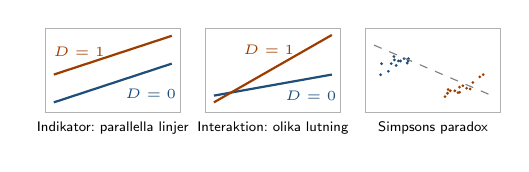
\begin{tikzpicture}[x=\figunit,y=\figunit,lab/.style={font=\fontsize{4.5}{5}\selectfont}]
\pgfmathsetseed{5}
\begin{scope}
  \miniram{Indikator: parallella linjer}
  \draw[hd,thick] (0.1,-0.38)--(1.5,0.08); \draw[ex,thick] (0.1,-0.05)--(1.5,0.41);
  \node[lab,hd] at (1.25,-0.28) {$D=0$}; \node[lab,ex] at (0.4,0.22) {$D=1$};
\end{scope}
\begin{scope}[xshift=1.9\figunit]
  \miniram{Interaktion: olika lutning}
  \draw[hd,thick] (0.1,-0.3)--(1.5,-0.05); \draw[ex,thick] (0.1,-0.38)--(1.5,0.42);
  \node[lab,hd] at (1.25,-0.3) {$D=0$}; \node[lab,ex] at (0.75,0.25) {$D=1$};
\end{scope}
\begin{scope}[xshift=3.8\figunit]
  \miniram{Simpsons paradox}
  \foreach \i in {1,...,14}{\pgfmathsetmacro\xx{0.15+0.5*rnd}\pgfmathsetmacro\yy{0.12+0.45*(\xx-0.4)+0.08*rand}\fill[hd] (\xx,\yy) circle (0.55pt);}
  \foreach \i in {1,...,14}{\pgfmathsetmacro\xx{0.9+0.5*rnd}\pgfmathsetmacro\yy{-0.22+0.45*(\xx-1.15)+0.08*rand}\fill[ex] (\xx,\yy) circle (0.55pt);}
  \draw[gray,dashed] (0.1,0.3)--(1.5,-0.3);
\end{scope}
\end{tikzpicture}
\end{center}

% ======================================================================
\sect[cBygg]{Polynom och transformationer}{sec:poly}
$Y=\beta_0+\beta_1X+\beta_2X^2+E$ är fortfarande en \emph{linjär} modell (linjär i parametrarna) ⇒ OLS. Används vid krökt samband (spridningsdiagram, krökta residualer); polynomen läggs till som separata variabler.\\
Effekten av $X$: $\mathrm d\hat y/\mathrm dx=b_1+2b_2x$ (beror på $x$); $b_2>0$ ⇒ U-form, $b_2<0$ ⇒ $\cap$-form; extrempunkt i $x=-b_1/(2b_2)$. Tolka termerna tillsammans. Behövs krökningen? $t$-test för $\beta_2$ (partiellt $F$ för flera högre termer).\\
\textbf{Centrering} $X_c=X-\bar x$: minskar korrelationen mellan $X$ och $X^2$ (VIF) och beräkningsproblem. Ändrar $b_0$, $b_1$ och deras tolkning ($b_1$ = lutningen vid $x=\bar x$), men \emph{inte} $b_2$, $\hat y$, residualerna, $\SSE$ eller $R^2$. Prediktion: centrera $x_0$ först!\\
\textbf{Transformera $Y$:} $\ln Y$ eller $\sqrt Y$ vid högerskeva residualer/ökande varians (tratt); $\ln X$ vid avtagande effekt. För hög polynomgrad ⇒ modellen följer bruset (överanpassning).

% ======================================================================
\sect[cDiag]{Avvikande och inflytelserika observationer}{sec:infl}
\begin{itemize}
\item \textbf{Residual} $e_i=y_i-\hat y_i$,\; $\mathrm{Var}(e_i)=\sigma^2(1-h_i)$.\quad \textbf{Standardiserad} $z_i=e_i/s$: antal standardavvikelser från residualernas medelvärde 0.
\item \textbf{Studentiserad (intern)} $r_i=\dfrac{e_i}{s\sqrt{1-h_i}}$.
\item \textbf{Jackknife} (externt studentiserad): residual från en modell anpassad \emph{utan} obs.\ $i$:\\
$r_{(-i)}=e_i\sqrt{\dfrac{n-k-2}{\SSE(1-h_i)-e_i^2}}=r_i\sqrt{\dfrac{n-k-2}{n-k-1-r_i^2}}\sim t_{n-k-2}$;\; $|r_{(-i)}|>2$–3 ⇒ avvikande i $Y$-led.
\item \textbf{Leverage} $h_i$ = diagonalen i $\mathbf H$: $0\le h_i\le1$, $\sum h_i=p$, medel $p/n$; avvikande i $X$-led om $h_i>2p/n$ (beror bara på $X$).
\item \textbf{DFFITS}$_i=r_{(-i)}\sqrt{\dfrac{h_i}{1-h_i}}$: inflytande på \emph{sitt eget} anpassade värde; gräns $|\text{DFFITS}|>1$ (små/medelstora data), $>2\sqrt{p/n}$ (stora data).
\item \textbf{Cook's} $d_i=\dfrac1p\cdot\dfrac{h_i}{1-h_i}\cdot r_i^2$: inflytande på \emph{alla} anpassade värden; gräns $d_i>1$, eller robust: värde ur Kleinbaum tabell A.10 ($n$, $k$, $\alpha$) delat med $n-(k+1)$.
\end{itemize}
Avvikande $Y$ nära $\bar x$ (lågt $h$) flyttar linjen lite; högt $h$ + avvikande $Y$ ⇒ stort inflytande; högt $h$ men på linjen ⇒ ofarlig.\\
\ex (2024-10-25, $n=20$ = litet): gräns 1 för båda; obs.\ 13: DFFITS $=-1.4$, Cook $=0.9$ ⇒ inflytelserik endast på sitt eget anpassade värde.\\
\ex (2025-02-28, $n\approx437$, $p=10$): DFFITS-gräns $2\sqrt{10/437}\approx0.30$; Cook $18.43/421\approx0.04$ ⇒ flera inflytelserika obs.\\
\textbf{Hantering:} (1) leta mät-/inmatningsfel; (2) undersök obs.:ens $X$- och $Y$-värden – vad särskiljer den?; (3) ta bara bort med motivering (fel, annan population) och redovisa; (4) börja med den mest inflytelserika – övriga mått ändras när den tas bort, anpassa om; (5) jämför modellen med/utan.

% ======================================================================
\sect[cDiag]{Multikollinearitet}{sec:vif}
Starka samband \emph{mellan} förklarande variabler. Följder: uppblåsta $s_{b_j}$ ⇒ icke-signifikanta $t$-test trots signifikant $F$; instabila skattningar, ”fel” tecken; $\SSq(X_2)\gg\SSq(X_2|X_1)$ (variablerna förklarar samma variation). Prediktioner och $R^2$ påverkas mindre.\\[1pt]
$\mathrm{VIF}_j=\dfrac{1}{1-R_j^2}$, $R_j^2$ från regression av $X_j$ på övriga $X$ (\emph{utan} $Y$). VIF $=5$ ⇔ $R_j^2=0.8$; VIF $=10$ ⇔ $R_j^2=0.9$.\\
\textbf{Tumregler:} enskilt VIF $>10$ eller medel-VIF $>5$ ⇒ hög risk. Parvis $|r|>0.9$ ⇒ överhängande risk (lösningsförslag). GVIF (kvalitativ variabel): $df=1$ ⇒ GVIF = VIF; annars jämför $\text{GVIF}^{1/(2df)}$ med $\sqrt5\approx2.24$ resp.\ $\sqrt{10}\approx3.16$.
Polynom/interaktioner ger artificiellt höga VIF – centrera och bedöm grundvariablerna (beräkna GVIF per grundvariabel).\\
\ex (2024-10-25) Antal bäddar (VIF 35.7), patienter/dag (37.8), sjuksköterskor (7.5) har $r=0.91$–$0.98$ sinsemellan ⇒ multikollinearitet; modell 2 saknar dem (låg risk), modell 1 har två kvar.\\
\textbf{Åtgärder:} ta bort en av de korrelerade variablerna, kombinera dem (kvot/index), centrera, samla mer data.

% ======================================================================
\sect[cGrund]{Studiedesign, confounding, Simpsons paradox}{sec:design}
\textbf{Observationsstudie:} vi observerar bara ⇒ endast korrelationssamband, inga kausala slutsatser. \textbf{Experiment:} forskaren styr $X$ (randomisering, kontroll) ⇒ kausala slutsatser möjliga. Korrelation ≠ kausalitet (filmer med Nicolas Cage mot drunkningar).
\textbf{Confounder} (störfaktor): variabel som påverkar både $X$ och $Y$ ⇒ skenbart/förvrängt samband. \textbf{Kontrollvariabel}: tas med i modellen för att justera (isolera) effekten av variabeln av intresse (t.ex.\ ålder och kön i en medicinstudie).\\
\textbf{Simpsons paradox:} ett samband som syns inom varje grupp försvinner eller byter riktning när grupperna slås ihop (näbbredd–näbblängd: positivt inom varje art, negativt totalt). Upptäck: färglägg spridnings-/residualdiagram efter grupp. Åtgärd: inkludera grupperingsvariabeln (ev.\ interaktion).\\
\ex (2025-02-28, uppg.\ 3) $e$ mot $\hat y$ markerat per art: Chinstrap har positiva residualer (underskattas), Gentoo negativa (överskattas) ⇒ art påverkar sambandet och bör ingå i modellen.

% ======================================================================
\sect[cBygg]{Modellval och validering}{sec:val}
{\small
\begin{tabular}{@{}>{\raggedright\arraybackslash}p{0.42\linewidth}>{\raggedright\arraybackslash}p{0.55\linewidth}@{}}
Mått & Bäst\\\hline
$R^2$ & högt – men ökar alltid, ej för modeller av olika storlek\\
$R^2_a$ & högt\\
$s=\sqrt{\MSE}$ & lågt\\
Mallows $C_p=\dfrac{\SSE_p}{\MSE_{\text{full}}}-(n-2p)$ & $C_p\approx p$ och litet (fulla modellen har alltid $C_p=p$)\\
$\mathrm{AIC}=n\ln(\SSE/n)+2(p+1)$ & lågt; straffar komplexitet, säger något om generaliserbarhet\\
$\mathrm{MSPR}=\frac1{n^*}\sum(y^*_i-\hat y^*_i)^2$ & lågt, på valideringsdata; $\mathrm{MSPR}\gg\MSE$ ⇒ överanpassad
\end{tabular}}\\[1pt]
($p$ = antal parametrar i delmodellen.) \textbf{Intern} validering: mått på träningsdata ($R^2_a$, AIC, $C_p$). \textbf{Extern}: dela data slumpmässigt i träning ($\ge50$\,\%) och validering ($\ge10$\,\%) och jämför MSPR; testmängd ger väntevärdesriktig skattning för den slutliga modellen; korsvalidering: $m$ grupper turas om. Tidsserier: dela vid en tidpunkt.
\textbf{Underanpassning}: för enkel, missar samband. \textbf{Överanpassning}: för komplex, modellerar bruset, generaliserar dåligt.\\
\textbf{Algoritmer:} best subsets (alla $2^k-1$ modeller), bakåteliminering (från full modell, tar bort), framåtval (från tom, lägger till), stegvis (båda). Giriga – ser ett steg i taget, ger \emph{inte} garanterat bästa modellen, känsliga för multikollinearitet, kan välja interaktion utan huvudeffekter. Bästa måttvärde ≠ lämplig modell ⇒ alltid residualanalys och test efteråt. Kvalitativa variabler hanteras som en grupp.\\
\ex (2025-01-20) Största modellen (9 var.) bäst på $R^2$ och $R^2_a$; modell 8 bäst på $C_p$ och AIC (straffar komplexitet ⇒ mer tillförlitliga för generaliserbarhet). Boyta–antal rum $r=0.815<0.9$ ⇒ ingen överhängande multikollinearitetsrisk.

% ======================================================================
\sect[cBygg]{Välj modell – checklista och ex.\ 2025-10-23, uppg.\ 2}{sec:valj}
(1) \textbf{Lämplighet:} residualdiagram (mönster, varians, normalitet, extremvärden). (2) \textbf{Anpassning mot komplexitet:} $R^2_a$, AIC, $C_p$, $s$ – välj den enklaste modell som förklarar i stort sett lika bra. (3) \textbf{Test:} $F$ för modellen, partiellt $F$ mellan nästlade modeller, $t$ för termerna. (4) \textbf{Multikollinearitet:} korrelationsmatris, VIF. (5) \textbf{Tolkningsbarhet} och hierarki. (6) \textbf{Prediktion} inom definitionsmängden.\\[1pt]
{\small
\begin{tabular}{@{}lrr>{\raggedright\arraybackslash}p{0.69\linewidth}@{}}
Modell & $k$ & $R^2_a$ & Bedömning\\\hline
mod\_1 & 5 & 0.918 & 5 huvudeffekter: krökt $e$ mot $\hat y$ (saknar interaktion); Tomtyta–Boendeyta $r=0.93$; Takhöjd och Tomtyta ej signifikanta\\
mod\_2 & 3 & 0.418 & utan Eluppvärmt: två grupper i $e$, S-formad QQ ⇒ viktig variabel saknas (Eluppvärmt, $r=0.74$ med $Y$)\\
mod\_3 & 15 & 0.945 & alla interaktioner upp till 4:e ordningen: bra residualer men överanpassad och svårtolkad\\
mod\_4 & 3 & 0.941 & Boendeyta × Eluppvärmt: slumpmässig svärm, rak QQ ⇒ \textbf{välj}
\end{tabular}}\\[1pt]
Partiellt $F$ (mod\_4 är nästlad i mod\_3): $F=\frac{(624\,728\,614-507\,449\,855)/12}{507\,449\,855/84}=1.62<F_{12,84;0.95}=1.87$ ⇒ extratermerna behövs inte. Modell-$F$ för mod\_4: $\frac{10\,260\,304\,836/3}{624\,728\,614/96}=525.6>F_{3,96;0.95}=2.70$. Interaktion $t=6.46>t_{96;0.975}=1.985$ ⇒ effekten av boendeyta är större för eluppvärmda (189.7 mot 113.5 kr/m$^2$); Eluppvärmt ($t=0.87$) behålls (hierarki). Prediktion (eluppvärmd, 200 m$^2$): $3604.88+113.54\cdot200+1857.10+76.15\cdot200=43\,400$ kr/år. Antal rum, takhöjd och tomtyta ingår inte i mod\_4 (tomtyta 1700 > max 1523 hade dessutom varit extrapolering).

% ======================================================================
\sect[cBygg]{Utvärdera en modell – ”Är modellen bra och lämplig?”}{sec:utvardera}
\textbf{Lämplig} = antagandena uppfyllda (§\ref{sec:modell}): normalfördelning (histogram, QQ), lika varians och linjäritet ($e$ mot $\hat y$), oberoende, extremvärden/inflytelserika observationer. \textbf{Bra} = högt $R^2$/$R^2_a$, signifikant $F$-test, rimliga och signifikanta koefficienter, ingen allvarlig multikollinearitet, lagom komplex. Avsluta med en samlad bedömning.\\
\ex (2025-02-28, 1d) ”Förklaringsgraden är hög ($\approx0.91$) och modellen är signifikant enligt $F$-testet. Residualerna är ungefär normalfördelade (klockformat histogram, QQ-punkterna följer linjen) men det finns många extremvärden i båda riktningarna. Variansen ökar med större anpassade värden ⇒ lika varians är inte uppfyllt. Extremvärdena bör undersökas (DFFITS, Cook's distance) och en transformation av $Y$ övervägas.”

% ======================================================================
\sect[cTenta]{Sant/falskt – påståenden från tidigare tentor}{sec:sf}
{\footnotesize Uppgiften: markera 2 korrekta resp.\ 2 falska påståenden; fel markering ger $-1$ p ⇒ markera bara det du är säker på. \sant = sant, \falskt = falskt.}
\begin{itemize}[leftmargin=7pt,labelsep=2pt]
\item[\falskt] $F$-test för modellen och partiellt $F$-test undersöker samma hypoteser. (Alla $\beta$ resp.\ en delmängd.)
\item[\falskt] Ett $t$-test kan avgöra om en kategorisk variabel med flera nivåer har samband med $Y$. (Partiellt $F$.)
\item[\sant] Kvantitativ variabel: ”när variabeln ökar en enhet förändras $Y$ med koefficientens värde” (givet övriga konstanta).
\item[\falskt] Kategorisk variabel tolkas som ”ökar med en enhet”. (Jämförelse mot referenskategorin.)
\item[\falskt] Normalfördelningen kontrolleras med histogram över responsvariabeln. (Över residualerna.)
\item[\sant] Stark korrelation mellan förklarande variabler riskerar problem med multikollinearitet.
\item[\sant] En kontrollvariabel justerar effekten av de andra variablerna för att hantera confounding.
\item[\falskt] Jackknife-residualer anger residualen i enheten ”standardavvikelser från residualernas medelvärde”. (Det gör standardiserade residualer.)
\item[\sant] En kvalitativ variabel modelleras med en indikatorvariabel färre än antalet kategorier.
\item[\sant] Polynom kan modellera icke-linjära samband i en linjär modell.
\item[\sant] $\SSq(X_2|X_1)$ beskriver hur mycket variation $X_2$ tillför en modell som redan innehåller $X_1$.
\item[\falskt] Pearsons korrelationskoefficient är alltid lämplig för att mäta styrkan i ett samband. (Bara linjära.)
\item[\falskt] Förklaringsgraden $R^2$ straffar modellen för antalet variabler. (Det gör $R^2_a$.)
\item[\sant] Den justerade förklaringsgraden straffar måttet utifrån antalet variabler i modellen.
\item[\falskt] En låg justerad förklaringsgrad visar på en bättre modell.
\item[\sant] Cook's distance visar om en observation har inflytande på alla anpassade värden.
\item[\sant] DFFITS visar om en observation har inflytande på sitt eget anpassade värde.
\item[\falskt] Framåtval, bakåteliminering eller stegvis regression leder alltid till den bästa modellen.
\item[\sant] Ett lägre AIC-värde är önskvärt när modeller jämförs.
\item[\falskt] Det enda sättet att bedöma en modells generaliserbarhet är extern validering. (T.ex.\ AIC.)
\item[\falskt] I en observationsstudie med två förklarande variabler är $\SSY=\SSq(X_1)+\SSq(X_2)+\SSE$. (Rätt: $\SSq(X_1)+\SSq(X_2|X_1)+\SSE$.)
\item[\sant] I enkel linjär regression testar $t$-testet för lutningen samma hypoteser som $F$-testet för modellen ($F=t^2$).
\end{itemize}
\textbf{Fler troliga påståenden:}
\begin{itemize}[leftmargin=7pt,labelsep=2pt]
\item[\sant] $R^2$ kan aldrig minska när en variabel läggs till.
\item[\sant] Sekventiella SS beror på variablernas ordning; $\SSE$ och $\SSR$ gör det inte.
\item[\falskt] Ett icke-signifikant intercept ska tas bort ur modellen.
\item[\sant] Prediktionsintervallet är bredare än konfidensintervallet för medelvärdet vid samma $x_0$.
\item[\falskt] Hög leverage innebär alltid att observationen är inflytelserik.
\item[\falskt] $p$-värdet är sannolikheten att $H_0$ är sann.
\item[\falskt] En observationsstudie kan påvisa kausala samband.
\item[\sant] Centrering minskar multikollinearitet mellan $X$ och $X^2$ utan att ändra $\hat y$ eller $R^2$.
\item[\falskt] Bonferroniintervall blir smalare ju fler intervall som skattas.
\item[\sant] Ett signifikant $F$-test betyder att minst en (inte alla) lutningsparametrar är skild från 0.
\end{itemize}

% ======================================================================
\sect[cBygg]{Utblick: logistisk regression och GLM (kap.\ 10–11)}{sec:glm}
Binär $Y$: $\pi=P(Y=1|X)$, logitlänk $\ln\frac{\pi}{1-\pi}=\mathbf x'\bb$ ⇔ $\pi=\frac{e^{\mathbf x'\bb}}{1+e^{\mathbf x'\bb}}$; skattas med maximum likelihood.
$e^{b_j}$ = oddskvot: oddset för $Y=1$ multipliceras med $e^{b_j}$ när $X_j$ ökar en enhet (övriga konstanta). Ingen SSE/$R^2$; Wald: $z=b_j/s_{b_j}\sim N(0,1)$.

% ======================================================================
\sect[cTenta]{Teorifrågor – korta modellsvar}{sec:teorisvar}
\textbf{När används polynom, och hur anpassas och tolkas de?} När sambandet mellan $X$ och $Y$ är icke-linjärt (krökt spridningsdiagram eller krökta residualer). Polynomtermerna ($X^2$, $X^3$, …) läggs till som separata variabler och modellen skattas med minsta kvadratmetoden (centrera gärna $X$). Effekten av $X$ tolkas genom att summera alla termers bidrag ($b_1+2b_2x$), inte en term i taget.\\
\textbf{Förklara Simpsons paradox.} Ett samband som syns inom flera grupper försvinner eller byter riktning när grupperna slås ihop, t.ex.\ positivt samband mellan näbbredd och näbblängd inom varje pingvinart men negativt totalt. Paradoxen kan dölja eller förvränga sambanden i en regressionsmodell ⇒ ta med grupperingsvariabeln.\\
\textbf{Varför justerad förklaringsgrad?} $R^2$ ökar alltid när variabler läggs till; $R^2_a$ straffar antalet parametrar och kan därför jämföra modeller av olika storlek.\\
\textbf{Varför inte $t$-test för en kategorisk variabel med flera nivåer?} Variabeln motsvaras av $c-1$ parametrar; varje $t$-test jämför bara en kategori med referensen (och beror på valet av referens). Hela variabeln testas med partiellt $F$-test, $H_0$: alla $c-1$ parametrar $=0$.\\
\textbf{KI eller PI?} KI skattar medelvärdet $\mu_{Y|x_0}$ (osäkerheten i linjen); PI gäller en enskild ny observation och innehåller även $\sigma^2$ ⇒ bredare, och krymper inte mot 0 när $n$ växer.\\
\textbf{Varför centrera?} Minskar korrelationen mellan $X$ och $X^2$ (eller interaktionstermer) ⇒ lägre VIF, stabilare skattningar och tolkbart $b_1$ (effekten vid $\bar x$); anpassningen ($\hat y$, $R^2$) är densamma.

% ======================================================================
\sect[cTenta]{Tentatips}{sec:tips}
\begin{itemize}
\item Svarsbladet: numeriska svar med tre decimaler; uträkningar och tolkningar på separat papper. Redovisa, tolka och motivera!
\item Saknas en siffra: skriv det, anta ett rimligt värde och lös vidare.
\item $df$: residual $n-(k+1)$; kvalitativ variabel med $c$ nivåer ger $c-1$ parametrar. Tabellavläsning och interpolering: §\ref{sec:tab}.
\end{itemize}

% ======================================================================
\sect[cTenta]{Vanliga fel att undvika}{sec:fel}
\begin{itemize}
\item Fel $df$: $\MSE=\SSE/(n-2)$ i enkel regression (inte $n-1$), allmänt $n-(k+1)$; i partiellt $F$ tas nämnarens $df$ från den \emph{kompletta} modellen.
\item Glömma ”i genomsnitt” och ”givet att övriga variabler hålls konstanta” i tolkningar.
\item Ej förkastad $H_0$ ≠ ”inget samband finns” – skriv ”inte tillräckligt stöd för …”.
\item Kontrollera normalfördelning på $Y$ i stället för på residualerna.
\item $t$-test för kategorisk variabel med flera nivåer, eller radernas $p$-värden i ANOVA-tabellen för flera variabler samtidigt (⇒ partiellt $F$).
\item Jämföra $R^2$ mellan modeller av olika storlek (⇒ $R^2_a$, AIC, $C_p$).
\item Ta bort en huvudeffekt som ingår i en interaktion eller ett polynom.
\item Blanda ihop KI (medelvärde) och PI (enskild observation).
\item Extrapolera utanför observerade $X$-värden; glömma att centrera $x_0$ när modellen är centrerad.
\end{itemize}

% ======================================================================
\sect[cTenta]{Tabellsamlingen – så läser du den}{sec:tab}
{\fontsize{7}{8}\selectfont\setlength{\tabcolsep}{1.6pt}\renewcommand{\arraystretch}{0.9}
Tabellsamlingen delas ut på tentan. \textbf{$t$-tabellen:} rad = $df$, kolumn = sannolikhet $q$ med $P(T\le t_{df;q})=q$ (tvåsidigt test/KI: $q=1-\alpha/2$; ensidigt: $q=1-\alpha$; Bonferroni: $q=1-\alpha/(2g)$). Vissa tabeller anger i stället svanssannolikheten $\alpha$ – läs rubriken: $t_{df;0.975}$ = kolumn 0.975 \textbf{eller} kolumn ”$\alpha=0.025$”.
\textbf{$F$-tabellen:} en tabell per $\alpha$; täljar-$df$ ($df_1$) i kolumner, nämnar-$df$ ($df_2$) i rader. \textbf{Normalfördelningen:} $z_{0.975}=1.96$, $z_{0.95}=1.645$ (= raden $df=\infty$ i $t$-tabellen).

\par\medskip
\noindent\begin{minipage}{\linewidth}
\textbf{Använda tabellerna.} Saknas exakt $df$: ta närmast \emph{lägre} $df$ (konservativt) eller interpolera linjärt i $1/df$: $q\approx q_1+(q_2-q_1)\dfrac{1/df-1/df_1}{1/df_2-1/df_1}$; t.ex.\ $F_{6,421;0.95}$ ligger mellan $df_2=200$ (2.14) och $500$ (2.12) ⇒ $\approx2.12$. Samband: $F_{1,df;1-\alpha}=t^2_{df;1-\alpha/2}$, $t_{\infty;q}=z_q$, $t_{df;\alpha}=-t_{df;1-\alpha}$.
\textbf{$p$-värde ur tabell:} se mellan vilka kolumner testvärdet hamnar, t.ex.\ $t=2.5$ med $df=20$: $2.086<2.5<2.528$ ⇒ $0.01<p<0.025$ ensidigt, $0.02<p<0.05$ tvåsidigt.
\end{minipage}

\par\medskip
\noindent\begin{minipage}{\linewidth}
\textbf{Normalkvantiler för QQ-plot för hand:} $z_{(i-0.5)/n}$ för $i=1,\dots,\lceil n/2\rceil$ (resten symmetriska: byt tecken). Plotta sorterade residualer mot dessa.\\
\begin{tabular}{@{}r|*{6}{r}@{}}
$n$ & $i=1$ & 2 & 3 & 4 & 5 & 6\\\hline
5 & $-$1.28 & $-$0.52 & 0.00 &  &  &  \\
6 & $-$1.38 & $-$0.67 & $-$0.21 &  &  &  \\
7 & $-$1.47 & $-$0.79 & $-$0.37 & 0.00 &  &  \\
8 & $-$1.53 & $-$0.89 & $-$0.49 & $-$0.16 &  &  \\
9 & $-$1.59 & $-$0.97 & $-$0.59 & $-$0.28 & 0.00 &  \\
10 & $-$1.64 & $-$1.04 & $-$0.67 & $-$0.39 & $-$0.13 &  \\
11 & $-$1.69 & $-$1.10 & $-$0.75 & $-$0.47 & $-$0.23 & 0.00 \\
12 & $-$1.73 & $-$1.15 & $-$0.81 & $-$0.55 & $-$0.32 & $-$0.10 \\
\end{tabular}
\end{minipage}
}

\end{multicols*}
\end{document}
